% Created 2012-04-13 Sex 15:26
\documentclass[11pt]{article}
\usepackage[utf8]{inputenc}
\usepackage[T1]{fontenc}
\usepackage{graphicx}
\usepackage{longtable}
\usepackage{hyperref}


\title{experiments}
\author{Rafael Lemes Beirigo}
\date{13 abril 2012}

\begin{document}

\maketitle

\setcounter{tocdepth}{3}
\tableofcontents
\vspace*{1cm}
\section{Experimento 00 Experimento da seção 4.3 do artigo: resolver task $\Omega$}
\label{sec-1}

\subsection{01 Utilizando $\Pi$$_1$, $\Pi$$_2$, $\Pi$$_3$, $\Pi$$_4$, $\Pi$$_5$}
\label{sec-1.1}

Esse experimento não está no artigo. Fiz para fins de testes.

\centerline{\includegraphics[width=10em]{/home/rafaelbeirigo/ql/experiments/00/01/map.png}}


\centerline{\includegraphics[width=10em]{/home/rafaelbeirigo/ql/experiments/00/01/w.png}}


\subsection{02 Utilizando $\Pi$$_2$, $\Pi$$_3$, $\Pi$$_4$}
\label{sec-1.2}

\centerline{\includegraphics[width=10em]{/home/rafaelbeirigo/ql/experiments/00/02/map.png}}


\centerline{\includegraphics[width=10em]{/home/rafaelbeirigo/ql/experiments/00/02/w.png}}


\subsection{03 Utilizando $\Pi$$_1$, $\Pi$$_2$, $\Pi$$_3$, $\Pi$$_4$}
\label{sec-1.3}

\centerline{\includegraphics[width=10em]{/home/rafaelbeirigo/ql/experiments/00/03/map.png}}


\centerline{\includegraphics[width=10em]{/home/rafaelbeirigo/ql/experiments/00/03/w.png}}


\subsection{04 Utilizando $\Pi$$_2$, $\Pi$$_3$, $\Pi$$_4$, $\Pi$$_5$}
\label{sec-1.4}

\centerline{\includegraphics[width=10em]{/home/rafaelbeirigo/ql/experiments/00/04/map.png}}


\centerline{\includegraphics[width=10em]{/home/rafaelbeirigo/ql/experiments/00/04/w.png}}


\subsection{Discussão}
\label{sec-1.5}

Q-Learning apresentou um desempenho superior ao de PRQ-Learning.
Posteriormente descobri que o motivo era que a tabela Q era reiniciada somente para o 
PRQ-Learning, o que prejudicava o desempenho desse algoritmo.


\section{Experimento 01}
\label{sec-2}

Repetição de 00 após correção do problema.
\subsection{01 Utilizando $\Pi$$_1$, $\Pi$$_2$, $\Pi$$_3$, $\Pi$$_4$, $\Pi$$_5$}
\label{sec-2.1}

\centerline{\includegraphics[width=10em]{/home/rafaelbeirigo/ql/experiments/00/01/map.png}}


\centerline{\includegraphics[width=10em]{/home/rafaelbeirigo/ql/experiments/01/01/w.png}}


\subsection{02 Utilizando $\Pi$$_2$, $\Pi$$_3$, $\Pi$$_4$}
\label{sec-2.2}

\centerline{\includegraphics[width=10em]{/home/rafaelbeirigo/ql/experiments/00/02/map.png}}


\centerline{\includegraphics[width=10em]{/home/rafaelbeirigo/ql/experiments/01/02/w.png}}


\subsection{03 Utilizando $\Pi$$_1$, $\Pi$$_2$, $\Pi$$_3$, $\Pi$$_4$}
\label{sec-2.3}

\centerline{\includegraphics[width=10em]{/home/rafaelbeirigo/ql/experiments/00/03/map.png}}


\centerline{\includegraphics[width=10em]{/home/rafaelbeirigo/ql/experiments/01/03/w.png}}


\subsection{04 Utilizando $\Pi$$_2$, $\Pi$$_3$, $\Pi$$_4$, $\Pi$$_5$}
\label{sec-2.4}

\centerline{\includegraphics[width=10em]{/home/rafaelbeirigo/ql/experiments/00/04/map.png}}


\centerline{\includegraphics[width=10em]{/home/rafaelbeirigo/ql/experiments/01/04/w.png}}


\subsection{Discussão}
\label{sec-2.5}

O PRQL apresenta um desempenho similar ao do QL.
O resultado não foi o esperado: esperava-se um desempenho melhor por parte do PRQL,
dado que esse possui a reutilização de políticas.
Hipótese: não está utilizando as políticas antigas


\section{Experimento 02 QL vs PRQL no mundo 05x05}
\label{sec-3}

Motivo: queria rodar o PRQL sem a parte PR, ou seja, só utilizando
QLearning, pra ver se estava tudo OK.

Nesse experimento, o PRQL NÃO utilizava $\pi$-reuse, somente QL

\centerline{\includegraphics[width=10em]{/home/rafaelbeirigo/ql/experiments/02/w.png}}


\subsection{Discussão}
\label{sec-3.1}

PRQL apresentou um desempenho bastante similar ao do QL, o que sugere que a execução
do PRQL sem $\pi$-reuse equivale à execução do QL.

Isso já era esperado, pois o elemento do PRQL que acelera o aprendizado é justamente
o $\pi$-reuse


\subsection{03 Repetição de 02, só que para o mundo 06x06}
\label{sec-3.2}

\centerline{\includegraphics[width=10em]{/home/rafaelbeirigo/ql/experiments/03/w.png}}


\subsection{Discussão}
\label{sec-3.3}

O resultado foi compatível com o obtido no experimento 02, conforme esperado


\subsection{04 Repetição de 02, só que para a task $\Omega$ do artigo}
\label{sec-3.4}

\centerline{\includegraphics[width=10em]{/home/rafaelbeirigo/ql/experiments/04/w.png}}


\subsection{Discussão:}
\label{sec-3.5}

   PRQL e QL apresentaram desempenhos compatíveis, o que era esperado


\subsection{05 Repetição de 04, só que dessa vez ativando o $\pi$-reuse}
\label{sec-3.6}

A bilioteca de políticas continha somente a $\Pi$^*_$\Omega$.

\centerline{\includegraphics[width=10em]{/home/rafaelbeirigo/ql/experiments/05/w.png}}

  Sucesso: PRQL acelerou QLearning


\subsection{06 Repetição de 05 para task $\Omega$ do artigo reutilizando $\Pi$$_2$, $\Pi$$_3$ e $\Pi$$_5$ (são as que mais ajudam o agente)}
\label{sec-3.7}

\centerline{\includegraphics[width=10em]{/home/rafaelbeirigo/ql/experiments/06/w.png}}



\subsection{09 Repetição de 02}
\label{sec-3.8}

\centerline{\includegraphics[width=10em]{/home/rafaelbeirigo/ql/experiments/02/w.png}}


\centerline{\includegraphics[width=10em]{/home/rafaelbeirigo/ql/experiments/09/w.png}}


\subsection{Discussão}
\label{sec-3.9}

O desempenho do PRQL aumentou em relação ao experimento 02. Isso pode
ser explicado pelo fato de que foi utilizado $\pi$-reuse nesse
experimento, o que contribui para acelerar o aprendizado.


\subsection{23 Repetição do 02}
\label{sec-3.10}



\subsection{10 Repetição de 09, mas reutilizando uma política ótima para o problema de chegar à localização oposta (pior política que poderia reutilizar)}
\label{sec-3.11}

\centerline{\includegraphics[width=10em]{/home/rafaelbeirigo/ql/experiments/09/w.png}}


\centerline{\includegraphics[width=10em]{/home/rafaelbeirigo/ql/experiments/10/w.png}}


\subsection{Discussão}
\label{sec-3.12}

O resultado foi de acordo com o esperado, pois o desempenho do PRQL
cai quando a política que está sendo reutilizada atrapalharia na
solução do problema.

\subsection{Discussão}
\label{sec-3.13}

O elevado desempenho do PRQL pode ser explicado pelo fato de que a
política utilizada é justamente a ótima para o problema.

\subsection{Discussão}
\label{sec-3.14}

Problema: plotando W[ 1]

Foi plotado somente a recompensa acumulada quando se reutilizava uma
das políticas possíveis, L[ 1]para uma das políticas
reutilizadas.

Como espera-se um aumento gradual da utilização da política $\Pi$$_{\mathrm{new}}$, e
a recompensa acumulada pela utilização de $\Pi$$_{\mathrm{new}}$ se encontra em W[
0], o valor plotado em W[ 1] não reflete o que esperamos.


\subsection{07 Repetição de 06}
\label{sec-3.15}

A repetição foi feita para testes

\centerline{\includegraphics[width=10em]{/home/rafaelbeirigo/ql/experiments/07/w.png}}


\subsection{Discussão}
\label{sec-3.16}

Problema: plotando W[ 1]
A repetição foi feita antes da detecção do problema descrito em 05.


\subsection{08 Repetição de 06, mas reutilizando somente a política ótima}
\label{sec-3.17}

\centerline{\includegraphics[width=10em]{/home/rafaelbeirigo/ql/experiments/08/w.png}}


\subsection{Discussão}
\label{sec-3.18}

O resultado foi diverso do esperado.

A recompensa acumulada estaciona em \~{} 0.13, um valor extremamente
baixo, superado pelo Q-Learning durante os experimentos.


\section{11 Resolver task $\Omega$ utilizando  $\Pi$$_2$, $\Pi$$_3$, $\Pi$$_4$, $\Pi$$_5$}
\label{sec-4}

\centerline{\includegraphics[width=10em]{/home/rafaelbeirigo/ql/experiments/11/w.png}}


\subsection{Discussão}
\label{sec-4.1}

PRQL apresenta desempenho inferior ao de QL, o oposto do esperado.


\subsection{12 Repetição de 11 reutilizando somente a policy obtida em 11 pelo QLearning (ótima para o problema)}
\label{sec-4.2}

\centerline{\includegraphics[width=10em]{/home/rafaelbeirigo/ql/experiments/12/w.png}}




\subsection{13 Repetição de 12, só que chamei o solveMDP\ldots{} pra criar os arquivos (tirar a dúvida se}
\label{sec-4.3}

  arquivos estão corretos)
\centerline{\includegraphics[width=10em]{/home/rafaelbeirigo/ql/experiments/13/w.png}}

Pude perceber a partir desse experimento que as políticas que estavam
sendo reutilizadas eram subótimas.


\subsection{14 Repetição do 13, só que agora utilizando a política ótima}
\label{sec-4.4}

\centerline{\includegraphics[width=10em]{/home/rafaelbeirigo/ql/experiments/14/w.png}}



\section{Obtenção das políticas ótimas para as tasks de 1 a 5}
\label{sec-5}

\subsection{15 Obtenção de $\Pi$$_1$}
\label{sec-5.1}

\centerline{\includegraphics[width=10em]{/home/rafaelbeirigo/ql/experiments/15/w.png}}

  Consumo de tempo: \~{} 10'


\subsection{16 Obtenção de $\Pi$$_2$}
\label{sec-5.2}

\centerline{\includegraphics[width=10em]{/home/rafaelbeirigo/ql/experiments/16/w.png}}

  Consumo de tempo: \~{} 10'


\subsection{17 Obtenção de $\Pi$$_3$}
\label{sec-5.3}

\centerline{\includegraphics[width=10em]{/home/rafaelbeirigo/ql/experiments/17/w.png}}

  Consumo de tempo: \~{} 10'


\subsection{18 Obtenção de $\Pi$$_4$}
\label{sec-5.4}

\centerline{\includegraphics[width=10em]{/home/rafaelbeirigo/ql/experiments/18/w.png}}

  Consumo de tempo: \~{} 10'


\subsection{19 Obtenção de $\Pi$$_5$}
\label{sec-5.5}

\centerline{\includegraphics[width=10em]{/home/rafaelbeirigo/ql/experiments/19/w.png}}

  Consumo de tempo: \~{} 10'


\section{20 Resolver task $\Omega$ utilizando $\Pi$$_2$, $\Pi$$_3$, $\Pi$$_4$, $\Pi$$_5$ (Repetição do 11)}
\label{sec-6}

\centerline{\includegraphics[width=10em]{/home/rafaelbeirigo/ql/experiments/20/w.png}}



\subsection{25 Repetição do 20}
\label{sec-6.1}



\section{21 Resolver task $\Omega$ utilizando $\Pi$$_2$, $\Pi$$_3$, $\Pi$$_4$}
\label{sec-7}

\subsection{26 Repetição do 21}
\label{sec-7.1}




\section{22 Resolver task $\Omega$ utilizando $\Pi$$_1$, $\Pi$$_2$, $\Pi$$_3$, $\Pi$$_4$}
\label{sec-8}

\subsection{24 Repetição do 22}
\label{sec-8.1}



\section{Aprendizado de $\Pi$_$\Omega$ com reutilização individual de políticas}
\label{sec-9}

\centerline{\includegraphics[width=10em]{/home/rafaelbeirigo/ql/experiments/27/map.png}}


\centerline{\includegraphics[width=10em]{/home/rafaelbeirigo/ql/experiments/27/w.png}}


No gráfico, os valores referentes ao Q-Learning foram obtidos no experimento 37.

\subsection{27 Reutilizando $\Pi$$_1$}
\label{sec-9.1}

Consumo de tempo: 5m20.356s
\subsection{28 Reutilizando $\Pi$$_2$}
\label{sec-9.2}

Consumo de tempo: 7m53.056s
\subsection{29 Reutilizando $\Pi$$_3$}
\label{sec-9.3}

Consumo de tempo: 9m8.582s
\subsection{30 Reutilizando $\Pi$$_4$}
\label{sec-9.4}

Consumo de tempo: 10m19.403s
\subsection{31 Reutilizando $\Pi$$_5$}
\label{sec-9.5}

Consumo de tempo: 6m8.686s


\section{Resolver task1 utilizando $\pi$-reuse($\Pi$$_1$)}
\label{sec-10}

\subsection{10 execuções}
\label{sec-10.1}

Política reutilizada: $\Pi$$_1$, obtida no experimento 15

w.32.png - dados do Q-Learning obtidos no experimento 32
\centerline{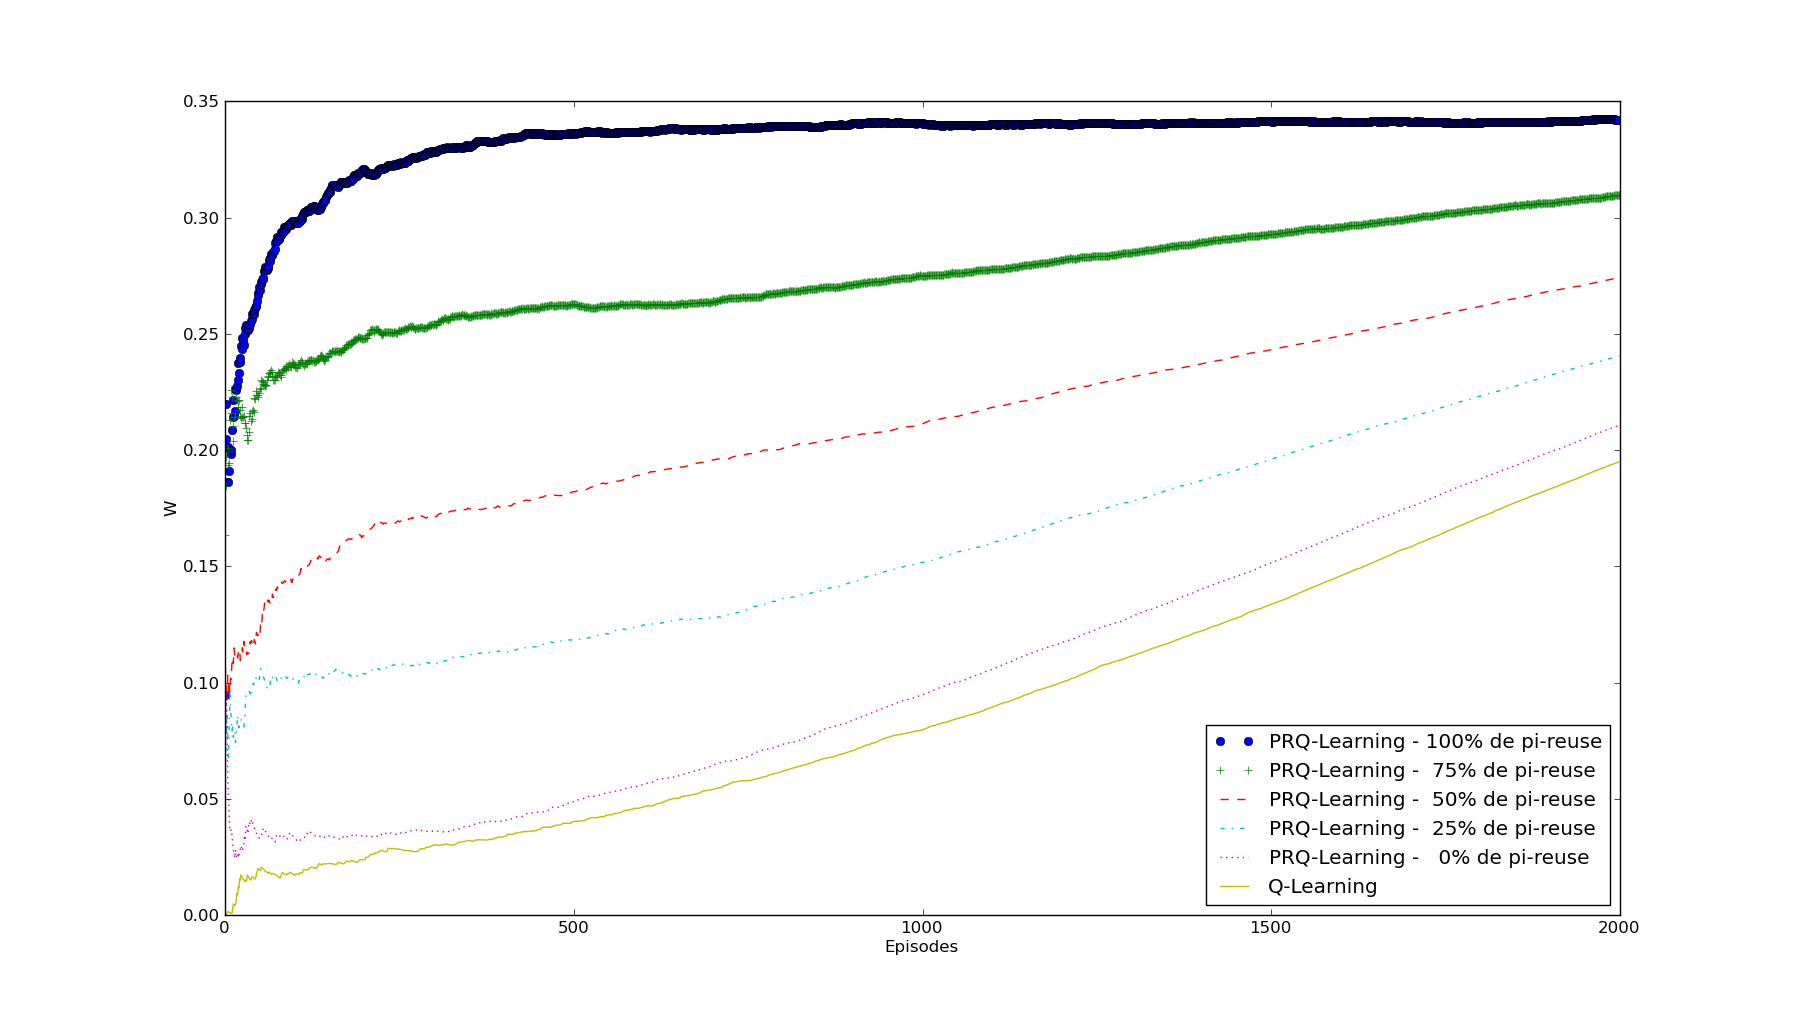
\includegraphics[width=10em]{/home/rafaelbeirigo/ql/experiments/32/w.32.png}}


w.37.png - dados do Q-Learning obtidos no experimento 37
\centerline{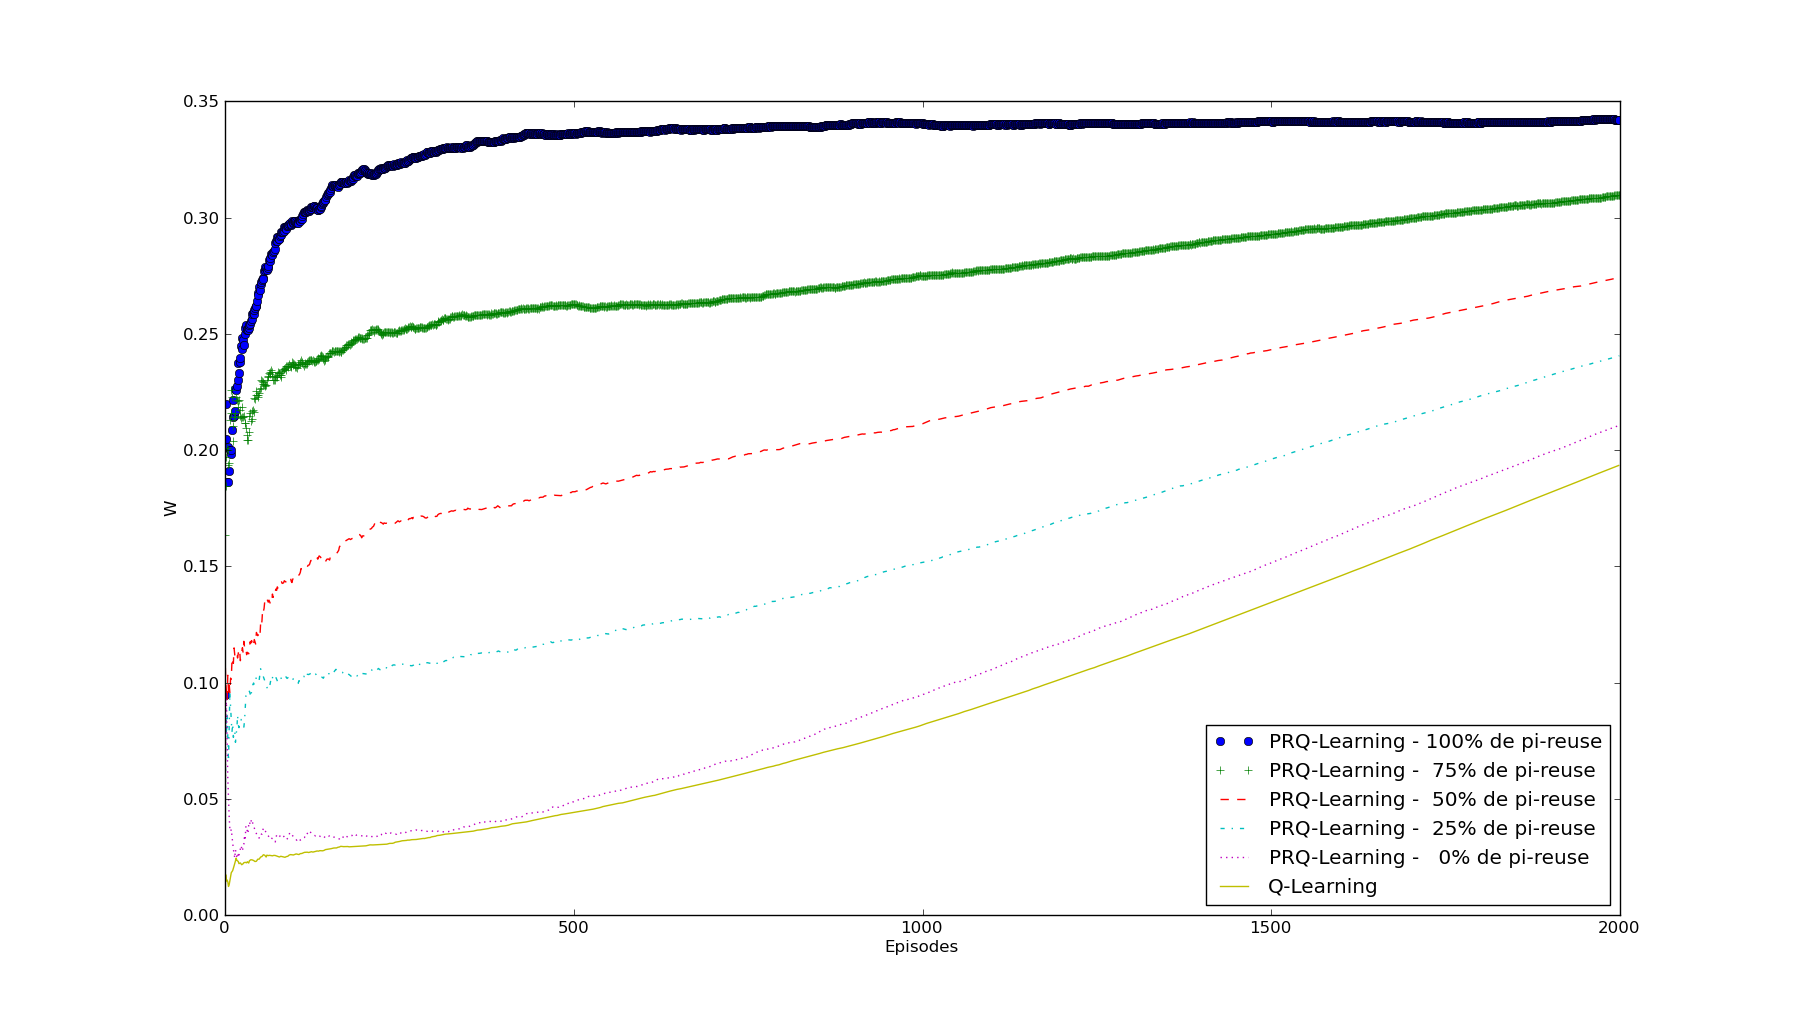
\includegraphics[width=10em]{/home/rafaelbeirigo/ql/experiments/32/w.37.png}}


\subsubsection{Experimento 32 - em 100\% dos episódios - 10 execuções}
\label{sec-10.1.1}

\subsubsection{Experimento 33 - em  75\% dos episódios - 10 execuções}
\label{sec-10.1.2}

\subsubsection{Experimento 34 - em  50\% dos episódios - 10 execuções}
\label{sec-10.1.3}

\subsubsection{Experimento 35 - em  25\% dos episódios - 10 execuções}
\label{sec-10.1.4}

\subsubsection{Experimento 36 - em   0\% dos episódios - 10 execuções}
\label{sec-10.1.5}


\subsection{100 execuções}
\label{sec-10.2}

\centerline{\includegraphics[width=10em]{/home/rafaelbeirigo/ql/experiments/37/w.png}}


Política reutilizada: $\Pi$$_1$, obtida no experimento 15

Dados do Q-Learning obtidos no experimento 37

\subsubsection{Experimento 37 - em   0\% dos episódios}
\label{sec-10.2.1}

\subsubsection{Experimento 38 - em  25\% dos episódios}
\label{sec-10.2.2}

\subsubsection{Experimento 39 - em  50\% dos episódios}
\label{sec-10.2.3}

\subsubsection{Experimento 40 - em  75\% dos episódios}
\label{sec-10.2.4}

\subsubsection{Experimento 41 - em 100\% dos episódios}
\label{sec-10.2.5}



\section{Testes da versão probabilística do PRQL (PRQL$_{\mathrm{prob}}$)}
\label{sec-11}

\subsection{PRQL$_{\mathrm{prob}}$ \emph{versus} PRQL}
\label{sec-11.1}

\subsubsection{Conservador: política determinística com 1.0 em tudo}
\label{sec-11.1.1}

Reutilizar uma política determinística ótima e sua versão probabilística (1.0 de probabilidade para cada ação ótima)

\begin{description}

\item[Task 1 reutilizando $\Pi$^*_1]\label{sec-11.1.1.1}


\centerline{\includegraphics[width=10em]{/home/rafaelbeirigo/ql/experiments/49/w.png}}


\begin{description}

\item[Experimentos]\label{sec-11.1.1.1.1}


\begin{description}

\item[49]\label{sec-11.1.1.1.1.1}


\begin{description}

\item[Algoritmo: PRQL$_{\mathrm{prob}}$]\label{sec-11.1.1.1.1.1.1}


\end{description}
\begin{description}

\item[Task: 1]\label{sec-11.1.1.1.1.1.2}


\end{description}
\begin{description}

\item[Políticas reutilizadas: $\Pi$$_1$^*_prob1]\label{sec-11.1.1.1.1.1.3}


\begin{description}

\item[$\Pi$$_1$^*_prob1 foi obtida colocando 1.0 em cada linha da política ótima determinística induzida por $\Pi$$_1$^*_prob]\label{sec-11.1.1.1.1.1.3.1}


\end{description}
\end{description}
\begin{description}

\item[Parâmetros: \href{file:///home/rafaelbeirigo/ql/experiments/49/PRQL/parameters.out}{/home/rafaelbeirigo/ql/experiments/49/PRQL/parameters.out}]\label{sec-11.1.1.1.1.1.4}



\end{description}
\end{description}
\begin{description}

\item[50]\label{sec-11.1.1.1.1.2}


\begin{description}

\item[Algoritmo: PRQL]\label{sec-11.1.1.1.1.2.1}


\end{description}
\begin{description}

\item[Task: 1]\label{sec-11.1.1.1.1.2.2}


\end{description}
\begin{description}

\item[Políticas reutilizadas: $\Pi$$_1$^*]\label{sec-11.1.1.1.1.2.3}


\end{description}
\begin{description}

\item[Parâmetros: \href{file:///home/rafaelbeirigo/ql/experiments/50/PRQL/parameters.out}{/home/rafaelbeirigo/ql/experiments/50/PRQL/parameters.out}]\label{sec-11.1.1.1.1.2.4}


\end{description}
\begin{description}

\item[Discussão:]\label{sec-11.1.1.1.1.2.5}


Os resultados corresponderam ao esperado, pois adicionar a probabilida
de 1.0 a cada ação da política determinística deveria gerar um resultado
equivalente na versão probabilística.


\end{description}
\end{description}
\end{description}
\end{description}
\begin{description}

\item[Task $\Omega$ reutilizando $\Pi$$_2$, $\Pi$$_3$, $\Pi$$_4$, $\Pi$$_5$]\label{sec-11.1.1.2}


\begin{description}

\item[PRQL]\label{sec-11.1.1.2.1}


\centerline{\includegraphics[width=10em]{/home/rafaelbeirigo/ql/experiments/27/w.png}}


\begin{description}

\item[Experimentos: 27 a 31]\label{sec-11.1.1.2.1.1}


\end{description}
\begin{description}

\item[Observações: Utilizando como referência aprendizado com QL do Experimento 37]\label{sec-11.1.1.2.1.2}




\end{description}
\end{description}
\begin{description}

\item[PRQL$_{\mathrm{prob}}$]\label{sec-11.1.1.2.2}


\begin{description}

\item[Experimentos: 51 a 55]\label{sec-11.1.1.2.2.1}


\centerline{\includegraphics[width=10em]{/home/rafaelbeirigo/ql/experiments/51/w.png}}



\end{description}
\end{description}
\end{description}
\subsubsection{Menos conservador: PRQL$_{\mathrm{prob}}$ vs QL}
\label{sec-11.1.2}

\begin{description}

\item[Task 1 cada vez mais probabilístico]\label{sec-11.1.2.1}


Utilização incremental de política probabilística ótima \emph{versus} \emph{péssima}
(PRQL$_{\mathrm{prob}}$ cada vez mais prob)

\begin{description}

\item[Algoritmo: PRQL$_{\mathrm{prob}}$]\label{sec-11.1.2.1.1}


\end{description}
\begin{description}

\item[Políticas reutilizadas:]\label{sec-11.1.2.1.2}


A partir de  $\Pi$$_1$, foi gerada uma nova política, em que para cada par estado-ação (s, a), geraram-se duas ênuplas:

\emph{s, a, p}

e

\emph{s, a^\{-1\}, (1 - p)}, em que 

\emph{a^\{-1\}} é a ação \emph{inversa} de \emph{a}, ou seja, se \emph{a} = \emph{East}, \emph{a^\{-1\}} = \emph{West}, se  \emph{a} = \emph{North}, \emph{a^\{-1\}} = \emph{South}, e assim por diante.

O valor de p varia por experimento, valendo \emph{0.1} no experimento \emph{56}, \emph{0.1} no experimento \emph{57}, e assim por diante, até atingir \emph{1.0} no experimento \emph{66}.

No experimento \emph{57}, \emph{a} vale \emph{0.0}, logo, a linha \emph{s, a, p} é omitida.

Um análogo disso ocorre para o experimento \emph{66}, onde \emph{p} vale \emph{1.0}, portanto \emph{1 - p} = \emph{0} e, dessa forma, a linha \emph{s, a^\{-1\}, (1 - p)} pode ser omitida.

Exemplo:

\emph{row1col1 East} \textbf{(linha original na $\Pi$$_1$)}

linhas geradas a partir dessa:

\emph{row1col1 East 0.7} \textbf{(ação ótima, por ter a maior probabilidade de escolha originalmente em $\Pi$$_1$ - 30\% de chance de ser a escolhida)}

\emph{row1col1 East 0.3} \textbf{(ação ``péssima'' - 70\% de chance de ser a escolhida)}

Ou seja, geramos políticas probabilísticas que variam da pior possível (a \emph{péssima}), que somente possui ações opostas àquelas da política ótima, até a ótima.

Intermediariamente, temos políticas ``sujas'', onde as ações ótimas são intercaladas por ações \emph{péssimas}.

Na tabela abaixo, temos a listagem completa dos valores de \emph{p} para cada experimento realizado.


\begin{center}
\begin{tabular}{rll}
 Experimento  &  Percentual de uso da ação \emph{ótima} (\emph{p})  &  Percentual de uso da ação \emph{péssima} \emph{(1 - p)}  \\
\hline
          56  &  0\%                                                &  100\%                                                    \\
          57  &  10\%                                               &  90\%                                                     \\
          58  &  20\%                                               &  80\%                                                     \\
          59  &  30\%                                               &  70\%                                                     \\
          60  &  40\%                                               &  60\%                                                     \\
          61  &  50\%                                               &  50\%                                                     \\
          62  &  60\%                                               &  40\%                                                     \\
          63  &  70\%                                               &  30\%                                                     \\
          64  &  80\%                                               &  20\%                                                     \\
          65  &  90\%                                               &  10\%                                                     \\
          66  &  100\%                                              &  0\%                                                      \\
\end{tabular}
\end{center}



\end{description}
\begin{description}

\item[Experimentos]\label{sec-11.1.2.1.3}


\begin{description}

\item[10 execuções]\label{sec-11.1.2.1.3.1}


\begin{description}

\item[56 a 66]\label{sec-11.1.2.1.3.1.1}


\centerline{\includegraphics[width=10em]{/home/rafaelbeirigo/ql/experiments/56/w.png}}


\begin{description}

\item[Parâmetros: \href{file:///home/rafaelbeirigo/ql/experiments/56/PRQL/parameters.out}{/home/rafaelbeirigo/ql/experiments/56/PRQL/parameters.out}]\label{sec-11.1.2.1.3.1.1.1}


\end{description}
\begin{description}

\item[QLearning: 56]\label{sec-11.1.2.1.3.1.1.2}


\end{description}
\begin{description}

\item[Discussão:]\label{sec-11.1.2.1.3.1.1.3}


Podemos verificar que a política que gerou o melhor resultado na reutilização
foi a que possui 70\% de \emph{ótimo} e 30\% de \emph{péssimo} ($\Pi$_\{70-30\}).

Isso foi uma surpresa, já que o natural seria esperar que a reutilização de
uma política que contenha somente ações ótimas gerasse um desempenho melhor
do que a reutilização de uma política que contivesse 30\% de ações \emph{péssimas}.

Entretanto podemos ver que a $\Pi$_\{70-30\} possui um \emph{jumpstart} significativo,
o que poderia jogar a média de W (que é justamente o que é mostrado no gráfico)
para cima.

Para testar se esse foi realmente o motivo, o experimento foi repetido, só que
dessa vez com 1000 execuções ao invés de 100 (experimentos de \emph{67} a \emph{77} e \emph{90}
a \emph{100}).

Com isso, esperamos diminuir o impacto que a \emph{sorte} de ter tido um bom
desempenho nos episódios iniciais pudesse ter sobre a recompensa média
alcançada.

Isso foi feito nos experimentos de \emph{67} a \emph{77}.

\end{description}
\end{description}
\begin{description}

\item[101 a 111]\label{sec-11.1.2.1.3.1.2}


\centerline{\includegraphics[width=10em]{/home/rafaelbeirigo/ql/experiments/101/w.png}}


\begin{description}

\item[Parâmetros: \href{file:///home/rafaelbeirigo/ql/experiments/101/PRQL/parameters.out}{/home/rafaelbeirigo/ql/experiments/101/PRQL/parameters.out}]\label{sec-11.1.2.1.3.1.2.1}


\end{description}
\begin{description}

\item[QLearning: 101]\label{sec-11.1.2.1.3.1.2.2}


\end{description}
\begin{description}

\item[Discussão:]\label{sec-11.1.2.1.3.1.2.3}


Esse experimento é uma repetição do \emph{56} a \emph{66}, para testar se está tudo OK.
O resultado correspondeu ao esperado.

\end{description}
\end{description}
\begin{description}

\item[112 a 122]\label{sec-11.1.2.1.3.1.3}


\centerline{\includegraphics[width=10em]{/home/rafaelbeirigo/ql/experiments/112/w.png}}


\begin{description}

\item[Parâmetros: \href{file:///home/rafaelbeirigo/ql/experiments/112/PRQL/parameters.out}{/home/rafaelbeirigo/ql/experiments/112/PRQL/parameters.out}]\label{sec-11.1.2.1.3.1.3.1}


\end{description}
\begin{description}

\item[QLearning: 112]\label{sec-11.1.2.1.3.1.3.2}


\end{description}
\begin{description}

\item[Discussão:]\label{sec-11.1.2.1.3.1.3.3}


Esse experimento foi realizado para testar se o \emph{merge} via \emph{git} do \emph{branch}
\emph{probabilistic} havia sido realizado com sucesso.

Os resultados estão muito próximos dos obtidos no mesmo experimento quando
executados com a versão anterior ao \emph{merge}, o que sugere que tenha ocorrido
tudo bem no processo de \emph{merge}.

\end{description}
\end{description}
\begin{description}

\item[123 a 133]\label{sec-11.1.2.1.3.1.4}


\centerline{\includegraphics[width=10em]{/home/rafaelbeirigo/ql/experiments/123/w.png}}


\begin{description}

\item[Parâmetros: \href{file:///home/rafaelbeirigo/ql/experiments/123/PRQL/parameters.out}{/home/rafaelbeirigo/ql/experiments/123/PRQL/parameters.out}]\label{sec-11.1.2.1.3.1.4.1}


\end{description}
\begin{description}

\item[QLearning: 123]\label{sec-11.1.2.1.3.1.4.2}


\end{description}
\begin{description}

\item[Discussão:]\label{sec-11.1.2.1.3.1.4.3}


Esse experimento foi realizado para testar se a estratégia de full-greedy implica
em alguma melhoria no desempenho do algoritmo.

O resultado esperado é que não haja melhorias, pelo contrário, que o fato de o
agente não poder realizar a exploração durante o episódio de Q-Learning implique
em uma queda do desempenho no aprendizado.

\end{description}
\end{description}
\end{description}
\begin{description}

\item[100 execuções]\label{sec-11.1.2.1.3.2}


\begin{description}

\item[79 a 89]\label{sec-11.1.2.1.3.2.1}


\centerline{\includegraphics[width=10em]{/home/rafaelbeirigo/ql/experiments/79/w.png}}


\begin{description}

\item[Parâmetros: \href{file:///home/rafaelbeirigo/ql/experiments/79/PRQL/parameters.out}{/home/rafaelbeirigo/ql/experiments/79/PRQL/parameters.out}]\label{sec-11.1.2.1.3.2.1.1}


\end{description}
\begin{description}

\item[QLearning: 79]\label{sec-11.1.2.1.3.2.1.2}



\end{description}
\begin{description}

\item[Discussão:]\label{sec-11.1.2.1.3.2.1.3}


O resultado correspondeu ao esperado.

\end{description}
\end{description}
\end{description}
\begin{description}

\item[1000 execuções]\label{sec-11.1.2.1.3.3}


\begin{description}

\item[67 a 77]\label{sec-11.1.2.1.3.3.1}


\centerline{\includegraphics[width=10em]{/home/rafaelbeirigo/ql/experiments/67/w.png}}


\begin{description}

\item[Parâmetros: \href{file:///home/rafaelbeirigo/ql/experiments/67/PRQL/parameters.out}{/home/rafaelbeirigo/ql/experiments/67/PRQL/parameters.out}]\label{sec-11.1.2.1.3.3.1.1}


\end{description}
\begin{description}

\item[QLearning: 67]\label{sec-11.1.2.1.3.3.1.2}


\end{description}
\begin{description}

\item[Discussão:]\label{sec-11.1.2.1.3.3.1.3}


O objetivo desse experimento era veriricar se o melhor desempenho obtido
com a reutilização de uma política com 30\% de ações \emph{péssimas} poderia
ser explicado por um desempenho extremamente bom no início, que jogaria
a média \emph{para cima}.

RESULTADOS: Podemos ver que os resultados corresponderam ao esperado, ou seja, quanto
mais probabilidade o agente tem de reutilizar uma ação ótima através do
$\pi$-reuse, melhor é o seu desempenho no aprendizado (medido pela média
cumulativa do \emph{W}).

Futuramente, pude ver que meu erro na verdade foi não ter percebido que
o experimento correspondente ao \emph{70-3-} na verdade terminou anormalmente.
Dessa forma, o \emph{w.out} plotado correspondia a um experimento realizado
anteriormente, o que explica seu comportamento de \emph{outlier}.

Através da análise do gráfico, podemos ver que uma adição igual ou superior
a 40\% de probabilidade de utilização de ações \emph{péssimas} implica em um
desempenho inferior ao da execução do QL.

\end{description}
\end{description}
\begin{description}

\item[90 a 100]\label{sec-11.1.2.1.3.3.2}


\centerline{\includegraphics[width=10em]{/home/rafaelbeirigo/ql/experiments/90/w.png}}


\begin{description}

\item[Parâmetros: \href{file:///home/rafaelbeirigo/ql/experiments/90/PRQL/parameters.out}{/home/rafaelbeirigo/ql/experiments/90/PRQL/parameters.out}]\label{sec-11.1.2.1.3.3.2.1}


\end{description}
\begin{description}

\item[QLearning: 90]\label{sec-11.1.2.1.3.3.2.2}


O resultado correspondeu ao esperado.


\end{description}
\end{description}
\end{description}
\end{description}
\end{description}
\section{IPMU}
\label{sec-12}

\subsection{42 Com arquivos originais - 2000 episódios, 100 passos}
\label{sec-12.1}

w.out completamente zerado.


\subsection{43 Com arquivos originais - 1e05 episódios, 1000 passos}
\label{sec-12.2}

Supondo que o problema relatado em 42 fosse a quantidade de episódios
e/ou passos, rodei novamente, com 


\subsection{44 Modifiquei o transitions.in}
\label{sec-12.3}

   Modificação realizada:
   Para cada linha do arquivo, o valor da transição foi alterado para
   1.0 / 136, sendo que 136 é o número total de estados.
Com isso, espero ter um grafo completo de transições, logo, poderei
   verificar se foi esse o problema que impediu o agente de receber
   recompensas nos experimentos 42 e 43.
Vale notar que estou supondo que existe uma linha s a s' t para todas
   as combinações de s a s' possíveis.
É bem provável que isso seja verdade já que a quantidade de linhas do
   arquivo transitions.in é 73984 = 136 * 4 * 136 (|S| * |A| * |S|).


\subsection{78 Reutilizando políticas probabilísticas}
\label{sec-12.4}

\centerline{\includegraphics[width=10em]{/home/rafaelbeirigo/ql/experiments/78/w.png}}


\subsubsection{PRQL}
\label{sec-12.4.1}

\begin{description}

\item[\emph{prob}: reutilizando pol. prob. enviada pelo Marcelo]\label{sec-12.4.1.1}


\begin{description}

\item[Algoritmo: PRQL$_{\mathrm{prob}}$]\label{sec-12.4.1.1.1}


\end{description}
\begin{description}

\item[Task: IPMU]\label{sec-12.4.1.1.2}


\end{description}
\begin{description}

\item[Políticas reutilizadas: $\Pi$$_{\mathrm{IPMU}}$\_{}prob]\label{sec-12.4.1.1.3}


\end{description}
\begin{description}

\item[Parâmetros: \href{file:///home/rafaelbeirigo/ql/experiments/78/PRQL/prob/parameters.out}{/home/rafaelbeirigo/ql/experiments/78/PRQL/prob/parameters.out}]\label{sec-12.4.1.1.4}



\end{description}
\end{description}
\begin{description}

\item[\emph{prob.det}: pol. ótima induzida pela pol. enviada pelo Marcelo]\label{sec-12.4.1.2}


\begin{description}

\item[Algoritmo: PRQL$_{\mathrm{prob}}$]\label{sec-12.4.1.2.1}


\end{description}
\begin{description}

\item[Task: IPMU]\label{sec-12.4.1.2.2}


\end{description}
\begin{description}

\item[Políticas reutilizadas: $\Pi$$_{\mathrm{IPMU}}$\_{}prob1 (1.0 para cada ação "ótima" (a que tinha a maior probabilidade no arquivo original))]\label{sec-12.4.1.2.3}


\end{description}
\begin{description}

\item[Parâmetros: \href{file:///home/rafaelbeirigo/ql/experiments/78/PRQL/prob.det/parameters.out}{/home/rafaelbeirigo/ql/experiments/78/PRQL/prob.det/parameters.out}]\label{sec-12.4.1.2.4}



\end{description}
\end{description}
\begin{description}

\item[\emph{det}: reutilizando pol. ótima induzida, só que na versão antiga do PRQL (a versão determinística)]\label{sec-12.4.1.3}


\begin{description}

\item[Algoritmo: PRQL]\label{sec-12.4.1.3.1}


\end{description}
\begin{description}

\item[Task: IPMU]\label{sec-12.4.1.3.2}


\end{description}
\begin{description}

\item[Políticas reutilizadas: $\Pi$$_{\mathrm{IPMU}}$\_{}det]\label{sec-12.4.1.3.3}


\end{description}
\begin{description}

\item[Parâmetros: \href{file:///home/rafaelbeirigo/ql/experiments/78/PRQL/det/parameters.out}{/home/rafaelbeirigo/ql/experiments/78/PRQL/det/parameters.out}]\label{sec-12.4.1.3.4}



\end{description}
\begin{description}

\item[Task: IPMU]\label{sec-12.4.2.1}


\end{description}
\begin{description}

\item[Parâmetros: \href{file:///home/rafaelbeirigo/ql/experiments/78/QL/parameters.out}{/home/rafaelbeirigo/ql/experiments/78/QL/parameters.out}]\label{sec-12.4.2.2}


\end{description}
\end{description}
\subsubsection{QL}
\label{sec-12.4.2}


\end{document}
